% !TEX root = ../../Noctua_Diplomarbeit.tex

\subsection{Handelsstrategien mit MAs} \label{subsection:mastrategie}

Eine simples Tradingmodell basiert auf einer einfachen �berkreuzung eines \gls{ma} �ber den Preis. Es wird dabei angenommen, dass ein Aufw�rtstrend eingesetzt hat, wenn der Preis �ber den \gls{ma} steigt, da der Kurs begonnen hat, schneller als der Durchschnitt zu steigen. Umgekehrt wird angenommen, dass bei einem Abfall des Kurses unter den \gls{ma} ein Abw�rtstrend folgt und daher wird ein Short-Signal generiert. Eine zus�tzliche Sicherheit ist gegeben, wenn der \gls{ma} selbst in die erwartete Kursrichtung dreht. (siehe \ref{fig:double_cross})

\begin{figure}
	\centering
		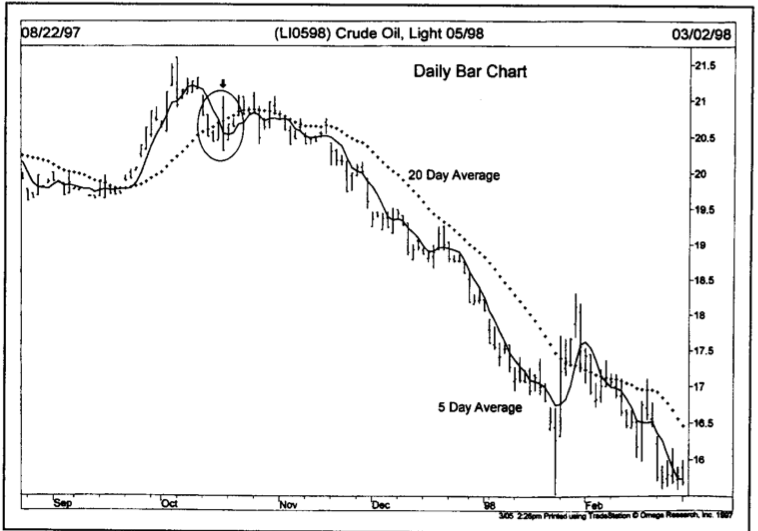
\includegraphics[width=0.8\textwidth]{graphics/fingrundlagen/double_cross.png}
	\caption[5,20 Double Cross Trading-System]{5,20 Double Cross Trading-System \cite{murphy-technische}}
	\label{fig:double_cross}
\end{figure}

Dieser simple Algorithmus hat einige Nachteile. Es ist zu jedem Zeitpunkt ein Signal gegeben, was bedeutet, dass immer entweder eine Long- oder eine Short-Position gehalten wird. Au�erdem verliert diese Strategie bei langen \glspl{ma} nach der Trendumkehr wieder viel vom Gewinn, da das Gegensignal erst sp�t generiert wird. Kurze \glspl{ma} erzeugen im Gegensatz oft Fehlsignale.\\

Eine h�ufiger verwendete Variante zur Signalgenerierung mit \glspl{ma} wird \emph{Double Crossover Method} genannt. Dabei kommen zwei unterschiedlich lange \glspl{ma} zum Einsatz, wobei ein Signal erzeugt wird wenn sich beide schneiden. Kreuzt der kurze \gls{ma} den l�ngeren entsteht ein Kaufsignal, auch \emph{Golden Cross} genannt, und vice versa. Diese Variante erzeugt weniger Fehlsignale als die direkte Verwendung des Preises, hinkt dem Markt daf�r aber auch st�rker hinterher. Die L�nge der Durchschnitte h�ngt wie immer sowohl vom Handelszeitraum und der gew�nschten Signalanzahl als auch vom Markt ab.

Dieses System kann noch um einen weiteren \gls{ma} erweitert werden. Der Einsatz dreier Durchschnitte, oder \emph{Triple Crossover Method}, verfeinert die Signalgenerierung nochmals. Einen beginnenden Aufw�rtstrend ist dann vorhanden, wenn der kurze \gls{ma} �ber dem mittleren liegt. Ein vollst�ndiges Kaufsignal entsteht sobald der kurze �ber dem mittleren, und jener wiederum �ber dem langen \gls{ma} notiert. Eine umgekehrte Anordnung ist als Verkaufssignal anzusehen. Auf diese Art kann beispielsweise bei unklaren Signalen eine Neutralstellung (i.e. keine Aktien im Portfolio) eingenommen werden oder die Market-Exposure (i.e. Anzahl der Aktien) reduziert werden. (siehe \ref{fig:triple_cross})
Normalerweise werden f�r solche Systeme \glspl{sma} verwendet, wobei aber besonders bei einem Double Crossover System die Anwendung eines \gls{ema},  \gls{dema} oder sogar \gls{tema} m�glich ist.

\begin{figure}
	\centering
		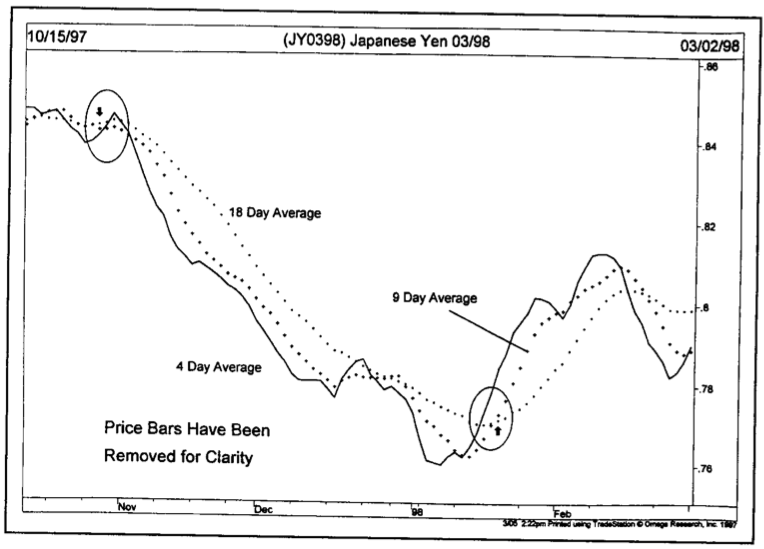
\includegraphics[width=0.8\textwidth]{graphics/fingrundlagen/triple_cross.png}
	\caption[4,9,18 Triple Cross Trading-System]{4,9,18 Triple Cross Trading-System \cite{murphy-technische}}
	\label{fig:triple_cross}
\end{figure}

\subsection{Fading-Strategie mit Bollinger B�ndern} \label{subsection:fading}

Seitw�rtsphasen zeichnen sich dadurch aus, dass der Preis mit einer gewissen Schwankungsbreite tendenziell weder steigt, noch sinkt. Bollinger B�nder sind hervorragend daf�r geeignet, diese Schwankungsbreite statistisch abzubilden, da sie um ein Vielfaches der Standardabweichung (normalerweise die doppelte) von Durchschnitt noch oben und unten versetzt liegen. Um in dieser Situation Gewinn zu erzielen, w�re es daher vorteilhaft, dann zu kaufen, wenn der Preis nahe dem unteren Bollinger Band nach oben dreht und umgekehrt, wenn der Preis nahe dem oberen Bollinger Band nach unten dreht, zu verkaufen --- kurz gesagt, tief kaufen und hoch verkaufen. In l�ngeren Seitw�rtsphasen l�sst sich mit dieser Strategie gut Gewinn erzielen. Wenn die Bewegung jedoch recht schnell wieder einen Trend ausformt, muss dies schnell erkannt werden, um nicht zu viel des bereits erzielten Gewinns wieder zu verlieren. Anzeichen f�r einen einsetzenden Trend k�nnen z.B. kontrahierende Bollinger B�nder oder ein niedriger ADX-Wert sein.